% --------------------------------------------
% LaTeX-Beamer-Vorlage des Arbeitsbereichs AmP
% Autor: Dipl.-Ing. Arthur Seibel ------------
% --------------------------------------------
%
% ----------------------------
% --------- Pr�ambel ---------
% ----------------------------
%
\documentclass[
%10pt
%11pt
%12pt
]{beamer} % Dokumentklasse
%\documentclass[draft]{beamer} % Entwickler-Modus in dem das File schneller kompiliert wird
%\documentclass[handout]{beamer} % Zum Ausdrucken besser geeignete Version der Folien
%\documentclass{article} % Artikel-Version; Funktioniert nur, wenn man zus�tzlich das Paket beamerarticle mittels 
%\usepackage{beamerarticle} % einbindet.
%
\usepackage{animate}
\usepackage[ansinew]{inputenc} % erweiterter Eingabezeichensatz (z.B. Sonderzeichen, Umlaute, etc.)
\usepackage[T1]{fontenc} % erweiterter T1 Zeichenvorrat
%\usepackage[ngerman]{babel} % Deutsche Trennregeln
\usepackage{booktabs} % Tabellenlayout
\usepackage{units} % einbinden von Einheiten
\usepackage{amsmath} % Matheumgebung
\usepackage{mathtools} % erweiterte Matheumgebung
\usepackage{dsfont} % f�r mathematische Mengensymbole
\usepackage{amssymb} % Symbolumgebung
\usepackage{theorem} % Erweiterung f�r Theoreme und S�tze
\usepackage{array} % f�r z.B. Matrizen
\usepackage{color} % Verwendung von Farben
\usepackage{rotate} % Drehung von Objekten
\usepackage{lmodern} % Serifenlose Schrift
\usepackage{tikz}    % TikZ Pictures 
\usepackage{graphics} % Einbindung von Grafiken in PS, PDF und JPG
\usepackage{epsfig} % Einbindung von Grafiken mit epsfig
\usepackage{pifont}
\usepackage{eurosym} % Verwendung des Euro-Zeichens
\usepackage{colortbl} % Tabellen farbig gestalten
\usepackage{xmpmulti}
\usepackage{multimedia}
%\usepackage{movie15}
\usepackage{pdfsync}
\usepackage{ulem} % f�r Unterstreichungen
\usepackage{url} % Internetlinks eingeben �ber \url{http://www.tu-harburg.de}
%
\usepackage{hyperref}
\usetheme{Madrid} % Pr�senthationsthema
\usecolortheme[RGB={45,198,214}]{structure} % Farbthema
\definecolor{tuhh}{RGB}{45,198,214} % Eigene Farbdefinition 
\useinnertheme{rounded} % Inneres Thema


%
% ----- Metainformationen -----
%

\setbeamercovered{transparent} % Transparente Overlays
\setbeamertemplate{frametitle}
{%
\vspace{-0.12ex}
\begin{beamercolorbox}[wd=\paperwidth,dp=0ex,ht=4ex,sep=0.5ex,colsep*=0pt]{frametitle}%
    \usebeamerfont{frametitle} \strut \insertframetitle  \hfill \raisebox{-2.5ex}[0pt][-\ht\strutbox ]{
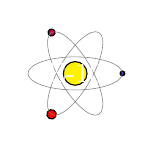
\begin{tikzpicture}[scale=.3]
\draw[color=black,fill=blue] (2,0) circle(.1);
\draw[help lines] (0,0)ellipse(2 and .7);
\begin{scope}[rotate=60]
\draw[color=black,fill=red] (-2,0) circle(.2);
\draw[help lines] (0,0)ellipse(2 and .7);
\end{scope}
\begin{scope}[rotate=120]
\draw[color=black,fill=purple] (2,0) circle(.15);
\draw[help lines] (0,0)ellipse(2 and .7);
\end{scope}
\draw[color=black,fill=yellow] (0,0)circle(.5)node[color=white]{E-10};
\end{tikzpicture}}
    \end{beamercolorbox}%
 }%
%
\title[simulation of a satellite trajectory]{Simulation of the trajectory of the satellite Galileo-FOC~FM4}
\author[Lars Schiller]{Lars Schiller}
\institute[E-10]{E-10-Simulation GmbH}
\date{\today}
% Alternativ kann mittels 
%\date{\today} % auch das aktuelle Datum eingetragen werden.
\titlegraphic{
\includegraphics[height=1cm]{TU-Logo.png}} % Logo unten zentriert
%
%% Inhaltsverzeichnis vor jedem Teilabschnitt:
%\AtBeginSection[]
%{
%  \begin{frame}<beamer>[noframenumbering]
%    \frametitle{�bersicht}
%    \tableofcontents[currentsection] % , subsection
%  \end{frame}
%}
%
% ---------- Dokument ----------
% ------------------------------
%
\begin{document}
%
%---------------------------------------
\begin{frame}%[noframenumbering]
\titlepage
\end{frame}


\begin{frame}
\frametitle{Problem description}
\begin{itemize}
\item Problem: simulate the trajectory of the satellite (subscripted by 3) with given initial conditions
\item mass afflicted bodies generate gravity forces to each other
\end{itemize}


\begin{center}
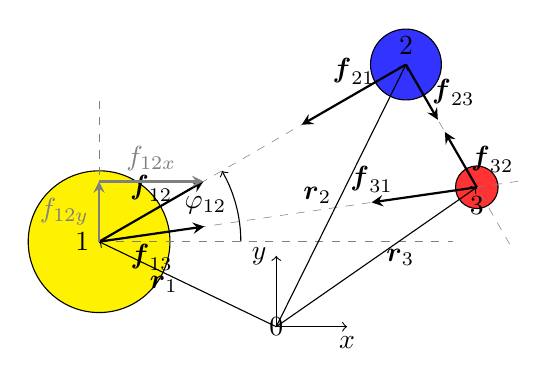
\begin{tikzpicture}[scale=.9]
%% Coordsys
\draw[->] (2.5,-1.2)coordinate(0)node{0}--++(1,0)node[below]{$x$};
\draw[->] (0)--++(0,1)node[left]{$y$};
%% Objects
\draw[fill=yellow] (0,0)circle(1)node[left]{1}coordinate(1);
\draw[fill=blue!80] (30:5)circle(.5)node[above]{2}coordinate(2);
\draw[fill=red!80] (2)++(-60:2)circle(.3)node[below]{3}coordinate(3);
%% Help Lines
\draw[help lines,dashed] (1)--++(5,0);
\draw[help lines,dashed] (1)--++(0,2);
\draw[help lines,dashed] (1)--++(30:5);
\draw[help lines,dashed] (1)--++(8.2:6);
\draw[help lines,dashed] (2)--++(-60:3);
%% Vecs
\draw[->] (0)--(1)node[midway,left]{$\boldsymbol{r}_1$};
\draw[->] (0)--(2)node[midway,left]{$\boldsymbol{r}_2$};
\draw[->] (0)--(3)node[midway,right]{$\boldsymbol{r}_3$};
%% Forces
\draw[thick,-stealth] (1)--++(30:1.7)node[above,midway]{$\boldsymbol{f}_{12}$};
\draw[thick,-stealth] (1)--++(8.2:1.5)node[below,midway]{$\boldsymbol{f}_{13}$};
\draw[thick,-stealth] (2)--++(210:1.7)node[above,midway]{$\boldsymbol{f}_{21}$};
\draw[thick,-stealth] (2)--++(-60:.9)node[right,midway]{$\boldsymbol{f}_{23}$};
\draw[thick,-stealth] (3)--++(180-60:.9)node[right,midway]{$\boldsymbol{f}_{32}$};
\draw[thick,-stealth] (3)--++(180+8.2:1.5)node[above]{$\boldsymbol{f}_{31}$};
\draw[thick,-stealth,gray] (1)--++(90:.5*1.7)node[midway,left]{${f}_{12y}$};
\pgfmathsetmacro{\l}{sqrt(3)/2*1.7}
\draw[thick,-stealth,gray] (1)++(90:.5*1.7)--++(0:\l)node[midway,above]{${f}_{12x}$};
\draw[->] (1)++(0:2)arc(0:30:2);
\path (1)++(15:2)node[left]{$\varphi_{12}$};
\end{tikzpicture}
\end{center}

\begin{equation}
\boldsymbol{f}_{ij} = \underbrace{\gamma \frac{m_im_j}{|\boldsymbol{r}_j-\boldsymbol{r}_i|^2}}_{\textnormal{magnitude}} ~ \underbrace{\frac{\boldsymbol{r_j}-\boldsymbol{r}_i}{|\boldsymbol{r_j}-\boldsymbol{r}_i|}}_{\textnormal{direction}} = \gamma \frac{m_im_j}{|\boldsymbol{r}_j-\boldsymbol{r}_i|^3} \left( \boldsymbol{r_j}-\boldsymbol{r}_i \right),
\label{eq:forces}
\end{equation}
\end{frame}

\begin{frame}
\frametitle{Mathematical model}

To obtain a system of ordinary differential equations use \textit{Newtons} 2nd Law:
\begin{equation}
m\ddot{r} = \sum\limits_n f_n.
\label{eq:newtons2nd}
\end{equation}
By defining the state vector $\boldsymbol{x}$ as:
$$
\boldsymbol{x} = \left[ r_{1x} ~~ r_{1y} ~~ r_{2x} ~~ r_{2y} ~~ r_{3x} ~~ r_{3y} ~~ \dot{r}_{1x} ~~ \dot{r}_{1y} ~~ \dot{r}_{2x}  ~~ \dot{r}_{2y} ~~ \dot{r}_{3x} ~~ \dot{r}_{3y} \right]^T
$$
equation ~\ref{eq:newtons2nd} can be written as
\begin{equation}
\dot{\boldsymbol{x}}
=
\left[
\begin{matrix}
\boldsymbol{x}(7:12) \\
\frac{1}{m_1} \left( f_{12x} + f_{13x} \right) \\
\frac{1}{m_1} \left( f_{12y} + f_{13y} \right) \\
\frac{1}{m_2} \left( f_{21x} + f_{23x} \right) \\
\frac{1}{m_2} \left( f_{21y} + f_{23y} \right) \\
\frac{1}{m_3} \left( f_{31x} + f_{32x} \right) \\
\frac{1}{m_3} \left( f_{31y} + f_{32y} \right) \\
\end{matrix}
\right]
\label{eq:ode}
\end{equation}
\end{frame}


\begin{frame}
\frametitle{Solving the Problem}
Solving of equation~\ref{eq:ode} with the advanced \textit{Euler}-method leads to:
\begin{center}
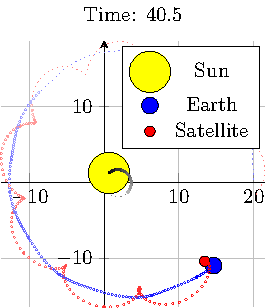
\includegraphics[width=.31\textwidth]{SolEuler/sol_odee_40_1e-3.pdf}
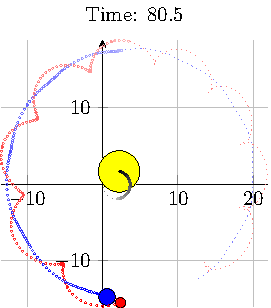
\includegraphics[width=.31\textwidth]{SolEuler/sol_odee_80_1e-3.pdf}
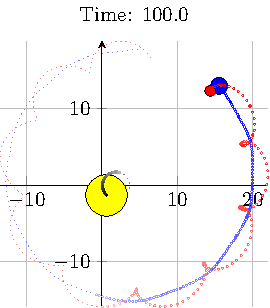
\includegraphics[width=.31\textwidth]{SolEuler/sol_odee_100_1e-3.pdf}
\end{center}

\end{frame}


\begin{frame}
\frametitle{Interpretation of the results}
\begin{itemize}
\item the trajectory of the satellite is stable
\item but a phase shift of the satellite can be observed, which is increasing by every rotation around the sun by the earth
\item by accepting this, a later control of the satellite will not be necessary

\end{itemize}
\end{frame}

\end{document}
%
